\begin{center}
	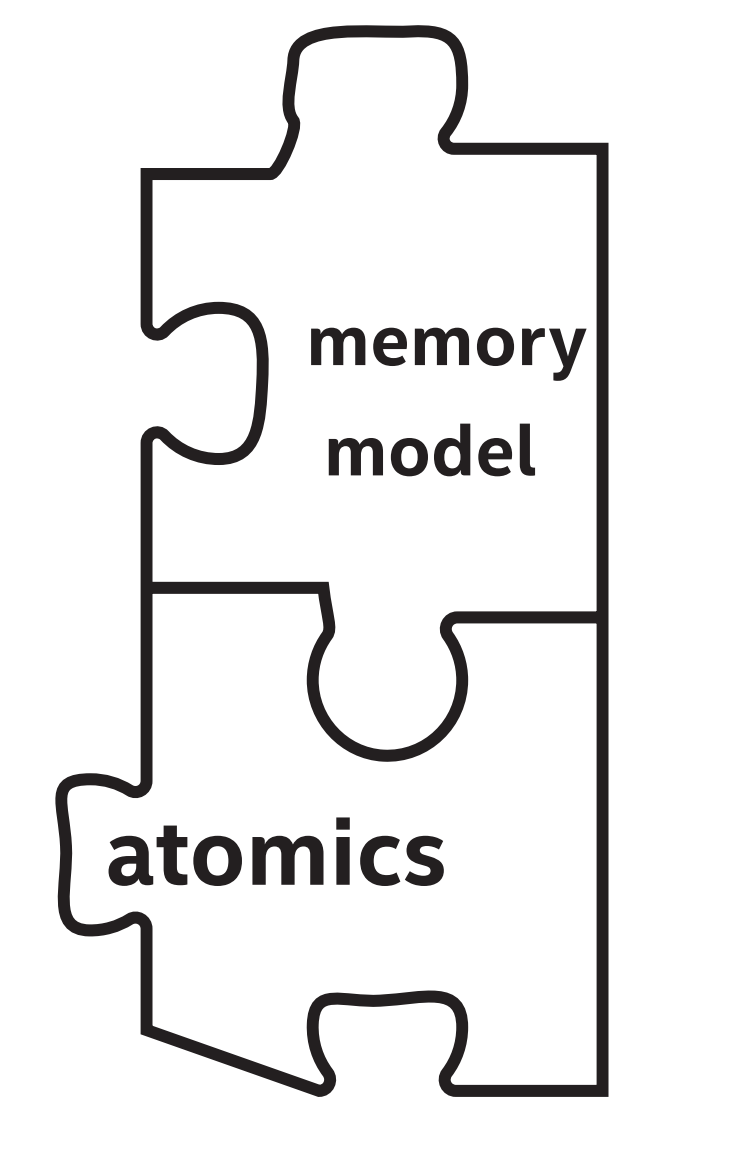
\includegraphics[width=0.5\textwidth]{content/chapter-19/images/1}
\end{center}

Memory consistency is not an esoteric concept if we want to be good parallel programmers. It is a critical piece of our puzzle, helping us to ensure that data is where we need it when we need it and that its values are what we are expecting. This chapter brings to light key things we need to master in order to ensure our program hums along correctly. This topic is not unique to SYCL or to DPC++.\par

Having a basic understanding of the memory (consistency) model of a programming language is necessary for any programmer who wants to allow concurrent updates to memory (whether those updates originate from multiple work-items in the same kernel, multiple devices, or both). This is true regardless of how memory is allocated, and the content of this chapter is equally important to us whether we choose to use buffers or USM allocations.\par

In previous chapters, we have focused on the development of simple kernels, where program instances either operate on completely independent data or share data using structured communication patterns that can be expressed directly using language and/or library features. As we move toward writing more complex and realistic kernels, we are likely to encounter situations where program instances may need to communicate in less structured ways—understanding how the memory model relates to DPC++ language features and the capabilities of the hardware we are targeting is a necessary precondition for designing correct, portable, and efficient programs.\par

The memory consistency model of standard C++ is sufficient for writing applications that execute entirely on the host device, but is modified by DPC++ in order to address complexities that may arise when programming heterogeneous systems and when talking about program instances that do not map cleanly to the concept of C++ threads. Specifically, we need to be able to\par

\begin{itemize}
	\item Reason about which types of memory allocation can be accessed by which devices in the system: using buffers and USM.
	\item Prevent unsafe concurrent memory accesses (data races) during the execution of our kernels: using barriers and atomics.
	\item Enable safe communication between program instances executing the same kernel and safe communication between different devices: using barriers, fences, atomics, memory orders, and memory scopes.
	\item Prevent optimizations that may alter the behavior of parallel applications in ways that are incompatible with our expectations: using barriers, fences, atomics, memory orders, and memory scopes.
	\item Enable optimizations that depend on knowledge of programmer intent: using memory orders and memory scopes.
\end{itemize}

Memory models are a complex topic, but for a good reason—processor architects care about making processors and accelerators execute our codes as efficiently as possible! We have worked hard in this chapter to break down this complexity and highlight the most critical concepts and language features. This chapter starts us down the path of not only knowing the memory model inside and out but also enjoying an important aspect of parallel programming that many people don’t know exists. If questions remain after reading the descriptions and example codes here, we highly recommend visiting the websites listed at the end of this chapter or referring to the C++, SYCL, and DPC++ language specifications.\par














































